\section{Noise and calibration}

\subsection{Noise in sensor systems}

Noise come from non-idealities of a signal that show
a strong temporal dependency.

Noise is \textbf{NOT} :
offset/gain error, saturation, component mismatch,
transfer function non linearity,\dots. A default specification is to keep the noise level below the value of the least significant bit (\SI{40}{\micro V} for \SI{2.5}{V} output converted by a 16 bits ADC).

The noise can be classified according to the following criterium:

\begin{itemize}
    \item \textbf{Source:} 
        \begin{itemize}
            \item Intrinsic from transducer or elements in conditioning circuit
            \item External/Environmental
        \end{itemize}
    \item \textbf{Nature:}
        \begin{itemize}
            \item Stochastic (random)
            \item Systematic (deterministic)
        \end{itemize}
    \item \textbf{Amplitude distribution:} 
        \begin{itemize}
            \item Gaussian
            \item Uniform
            \item Bounded
        \end{itemize}
    \item \textbf{Spectrum:}
        \begin{itemize}
            \item White
            \item Colored
            \item Periodic
        \end{itemize}
\end{itemize}


\subsubsection{White/Thermal noise}

\begin{mydef}
White noise is an intrinsic random noise arising from the discrete
nature of electrical charges (random
Brownian motion of electrons). It is a random signal having equal intensity at different frequencies, giving it a constant power spectral density
\end{mydef}

The noise power in a resistor is given by: $\overline{e_n}^2 = 4k TR\Delta f$ [\si{V^2}]. It increases with the resistance, the temperature and $\Delta f$ the bandwidth over which the measurement is made. \textbf{The noise of multiple resistors add up.} (when they are expressed in \si{V^2}).

The same effect can be observed with semiconductors (junctions, BJT, MOSFET) and is called in this case the \textit{shot noise}. Finally it also appears when sampling a voltage on a capacitor, this is the \textit{kT/C noise}.

\subsubsection{Pink/Flicker noise}

\begin{mydef}
Pink noise is an intrinsic random noise appearing at low frequencies.
\end{mydef}

\begin{minipage}{0.45 \linewidth}
Dominates usually below 100 Hz $\rightarrow$ critical for sensors. It is highly dependent on the quality of the semiconductor
manufacturing process.

It can be observed as a $1/f$ trend on the spectrum analysis of the sensor.
\end{minipage}\hfill
\begin{minipage}{0.45 \linewidth}
\begin{figure}[H]
    \centering
    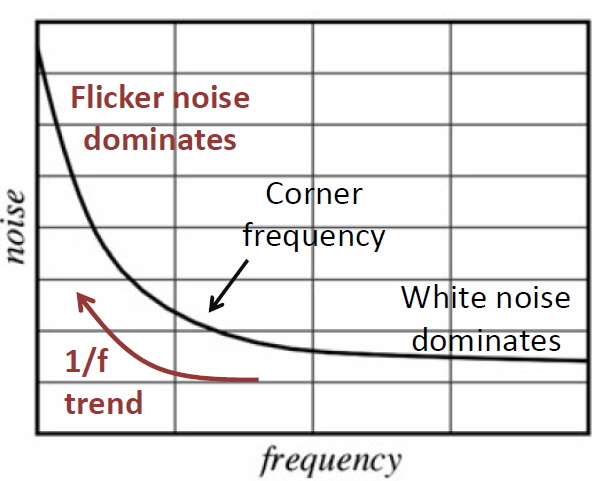
\includegraphics[width = 0.7\textwidth]{L3/img/pink-noise.PNG}
\end{figure}
\end{minipage}

\subsubsection{Environmental noises}

\begin{itemize}
    \item Random or systematic
    \item Usually periodic
\end{itemize}

Examples : gravitation field, magnetic field of the Earth, humidity, thermal variations, \dots

\begin{figure}[H]
    \centering
    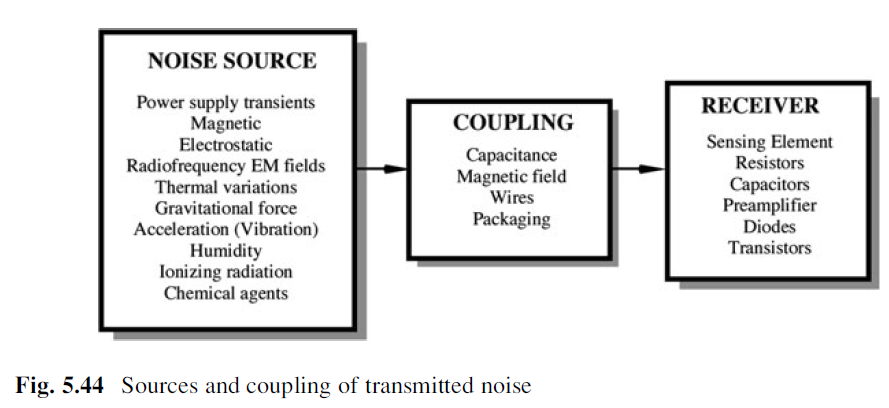
\includegraphics[width = 0.8\textwidth]{L3/img/environmental-noise.PNG}
\end{figure}

\subsubsection{Crosstalk noise}

Crosstalk noise is a coupling of both external and internal noise
sources to noise-sensitive components in the
circuits through parasitic capacitances (External: human-to-ground cap $\approx$ 700 pF, Internal: pin-to-pin cap in integrated circuits $\approx$ 2 pF)

\subsubsection{Seebeck noise}

This noise is a result of the Seebeck effect which is manifested as the generation of an electromotive force (emf) when two dissimilar metals are joined together. This noise is usually $< \SI{10}{\micro V}$.

\subsubsection{Noise expression}

The noise can be expressed in:
\begin{itemize}
    \item Volts (before the digitization)
    \item LSBs (after the digitization)
    \item The units of the physical domain (input-referred noise)
    \item SNR: ratio between the sensor signal and the noise (in dB)
\end{itemize}
The noise is either characterized by:
\begin{itemize}
    \item The peak-to-peak value for deterministic sources
    \item or better expressed with its RMS value for stochastic sources (assuming a Gaussian distribution)
\end{itemize}
If the measurement bandwidth is not fixed, the noise is expressed by its Power Spectral Density
(e.g. \si{V/\sqrt{Hz}} or \si{V^2/Hz}) assuming a white spectrum. 

The noise can impact the output signal in two different ways: 

\begin{itemize}
    \item \textbf{Additive noise}: noise magnitude is independent on the signal level
    \item \textbf{Multiplicative noise}: noise is modulated by the signal (strongly alters the transfer function)
\end{itemize}

\subsubsection{Input Referred Noise}

It allows to quantitatively compare the impact
of noise sources on the measurement error. It is expressed in the scale of the physical signal to
measure such that we bring back each each noise source to the input by taking into account the gains of different stages.

\begin{figure}[H]
    \centering
    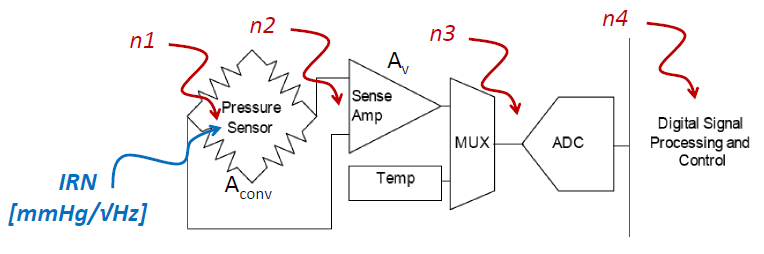
\includegraphics[width = 0.8\textwidth]{L3/img/reffered-noise.PNG}
\end{figure}

Input Referred Noise: $e_{IRN} = \sqrt{e_{n1}^2 + (e_{n2}/A_{conv})^2 + (e_{n3}/(A_v A_{conv}))^2  + (0\times e_{n4}) ^2}$. There is no noise for a digital signal.

\subsection{Calibration}

Transfer functions can vary because of:
\begin{itemize}
    \item  manufacturing tolerances
    \item second-order environmental parameters (temperature)
\end{itemize}
When the variations in the transfer function
or in the signal conditioning chain is higher than the required accuracy $\rightarrow$ calibration.

A usual calibration is performed as follows:

\begin{enumerate}
    \item Start with an approximate transfer function
    \item Matching pairs of reference input stimuli with
observed output signals (calibration points)    
    \item Recover the real inverse transfer function and
store the unknown parameters
\end{enumerate}
The challenge of calibration is the following:

\begin{itemize}
    \item In low-volume production, the calibration is not time consuming, but the equipment will be expensive
    \item In high-volume production, the calibration will be time consuming
\end{itemize}
Some techniques are available to calibrate a sensor:

\begin{enumerate}
   \item Modification (\textbf{trimming}) of the sensor properties to
fit the predetermined transfer function (e.g. remove matter from a thermistor to change its resistance) 
    \item Creating a sensor-specific reference device with
matching properties at particular calibrating points. (e.g. choose a matching resistor to build a Wheatstone bridge)
    \item Adjustment of the data acquisition system to trim
the measured data by making them to fit into a
normalized or \textit{ideal} transfer function.
\end{enumerate}

    
